\chapter{面向云原生应用权限提升漏洞的自动化防控技术报告}

\section{背景与问题}

Kubernetes 系统凭借其自动化管理与弹性伸缩能力，已成为容器编排领域的事实标准。在持续集成/持续部署、服务治理、可观测性与功能拓展需求驱动下，生产环境常引入 Prometheus、Jenkins、Istio 等第三方开源应用。此类组件的接入通常需要授予其访问 Kubernetes 资源（如 Pods、Secrets、Services）的权限以保障功能正常运行，但也带来权限配置不当与权限边界失控的风险。

攻击者可能利用第三方应用及其依赖库中的高危漏洞劫持容器并获得基础权限，进而借助过度开放的 ServiceAccount、缺乏最小权限约束的 ClusterRole 等配置不当问题发起权限提升攻击，最终威胁集群整体安全。例如 \texttt{CVE-2024-56513}、\texttt{CVE-2022-29179} 等事件表明，漏洞利用与权限配置错误往往呈链式叠加效应，使“快速缓解”在补丁完全可用之前成为必要环节。

另一方面，漏洞的安全响应存在显著滞后：部分高危漏洞的完全修复周期可长达数年。统计结果显示，仅约 61.8\% 的 Kubernetes 开源应用权限提升高危漏洞在公开前完成修复，且仅约 18\% 的漏洞能够在公开前至少 7 天得到修复，为用户留出更新迁移与风险缓解的缓冲时间；同时在漏洞上报、漏洞公开与漏洞修复之间也存在不同程度的延迟。

在此情境下，大模型为 CVE 的快速缓解与防控提供了关键的智能化支撑：其一，利用语义理解能力从公告、代码与讨论材料中提取与权限边界相关的关键信息，缩短人工阅读与归纳的时间；其二，在证据约束与结构化输出要求下，生成可解释、可执行的候选缓解策略，从而加速“分析—生成—筛选—交付”的闭环。

\subsection{权限提升漏洞的分类}

权限提升漏洞是指攻击者利用应用或系统中的安全缺陷，获得超过其当前权限级别的访问能力，从而实施越权操作或扩大攻击影响。针对 Kubernetes 容器化应用的权限提升攻击方式与威胁模型呈现多元化。为便于将漏洞特征映射到可实施的控制域（例如身份与权限、网络隔离、运行时检测与审计），本文采用基于根本成因的分类视角，对常见路径进行归纳总结，如图\ref{fig:vulnerability-taxonomy} 所示。

\begin{figure}[h]
    \centering
    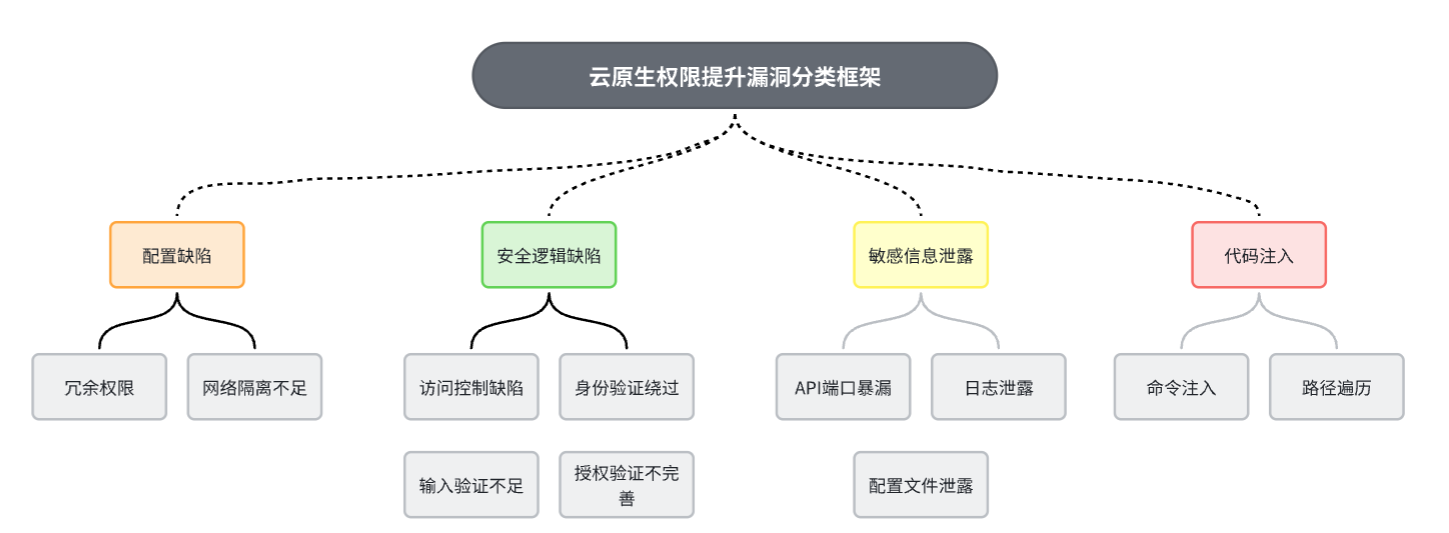
\includegraphics[width=0.95\textwidth]{images/vulnerability_taxonomy.png}
    \caption{Kubernetes 容器化应用权限提升攻击方式分类}
    \label{fig:vulnerability-taxonomy}
\end{figure}

\textbf{1. 配置缺陷}：应用或基础设施的配置不当导致的安全漏洞，包括：
\begin{itemize}
    \item 权限配置过宽：Kubernetes RBAC配置不当、IAM策略权限过大等，允许低权限用户获得高权限访问；
    \item 网络隔离不足：容器、Pod或服务间缺乏网络隔离，导致攻击者可以横向移动获取其他权限上下文。
\end{itemize}

\textbf{2. 安全逻辑缺陷}：应用代码中的安全机制设计或实现不当，包括：
\begin{itemize}
    \item 访问控制缺陷：应用的权限检查不完全或存在逻辑漏洞，允许绕过权限验证；
    \item 身份验证绕过：认证机制设计缺陷，攻击者可以冒充他人身份或跳过认证步骤；
    \item 授权验证不完善：权限检查在某些操作路径或边界条件下缺失。
\end{itemize}

\textbf{3. 敏感信息泄露}：重要的身份、密钥或权限信息意外暴露，包括：
\begin{itemize}
    \item API端口暴露：管理接口、内部API或调试端口未受保护暴露在网络上；
    \item 日志泄露：日志文件包含敏感信息（如token、密钥、命令历史）；
    \item 配置文件泄露：配置文件包含硬编码的凭证或密钥。
\end{itemize}

\textbf{4. 代码注入}：应用对用户输入的处理不当，允许注入恶意代码，包括：
\begin{itemize}
    \item 命令注入：应用直接执行用户提供或可控的命令，攻击者可以执行任意系统命令；
    \item 路径遍历：应用文件访问检查不完整，攻击者可以访问系统其他部分的文件。
\end{itemize}



\subsection{动机与挑战}

在云原生场景下，漏洞补丁的发布与升级往往存在时间差；同时，生产环境的组件组合与权限边界具有显著异构性。对于权限提升类漏洞而言，这意味着处置流程通常需要在“补丁尚不可用或难以及时部署”的阶段，先采取\textbf{临时防控}措施以降低风险暴露面。基于这一现实需求，本文将动机聚焦于可动态下发的安全控制域，通过准入控制、网络隔离与运行时检测等手段，对攻击链中的关键环节施加约束，实现可快速部署、可验证、可回滚的风险缓解。

为便于将上述动机具体化，本文将常见动态控制与工具能力归纳为如下可落地控制点：
\begin{itemize}
    \item \textbf{准入与策略约束}：基于 \texttt{OPA/Gatekeeper} 或 \texttt{Kyverno} 等准入策略，对特权容器、宿主机路径挂载、高风险 Linux \texttt{capabilities}、过宽 RBAC 绑定等高风险资源进行阻断或强制修正；
    \item \textbf{网络隔离与最小连通}：基于 \texttt{NetworkPolicy} 对命名空间与工作负载间通信进行白名单化，限制横向移动与数据外传路径；
    \item \textbf{运行时检测与响应}：基于 \texttt{Falco} 等运行时安全工具，监测异常系统调用、提权相关行为与逃逸迹象，并结合告警、隔离等处置流程降低影响扩散；
    \item \textbf{安全基线与最小权限}：结合 Pod 安全基线（如 \texttt{Pod Security Standards}）与账户/令牌治理，压缩默认配置下的权限暴露面。
\end{itemize}

面向权限提升漏洞的临时防控，自动化生成的方案需要同时满足三个要求：\textbf{可解释}（能够说明措施与风险点的对应关系）、\textbf{可执行}（给出可落地步骤，并明确验证与回滚边界）、\textbf{可复核}（关键结论可回溯到证据与环境假设）。然而，漏洞描述与运行环境信息往往存在噪声与缺失，不同控制手段对业务的副作用也存在差异，使得“生成—筛选—交付”难以依靠单一的启发式规则完成。为此，本文采用结构化产物、证据来源追踪与规则化质量评价相结合的方式，将策略生成过程约束到可检查的中间结果上，降低不确定性对交付质量的影响。

在上述约束下，引入大模型的主要考虑在于提升“信息理解与候选生成”的效率与覆盖度。面对公告、代码与讨论材料等多源非结构化证据，大模型可在检索增强上下文的支持下，归纳漏洞成因，梳理权限边界与可控点，并生成多种候选的临时防控方案。与此同时，本文通过结构化字段、动作序列规范与门槛评价，将生成结果转化为可检查、可复核的交付产物，使其更适用于 CVE 的快速缓解与防控流程，并与必要的验证与审计环节保持一致。


本文面向云原生权限提升漏洞的临时防控需求，构建一套以“证据约束 + 结构化产物 + 质量评价”为核心的自动化策略生成流程。整体框架由三个阶段组成：

{\bfseries （1）开源应用知识库构建}：从收到权限提升高危漏洞威胁的云原生开源应用的源代码、Issue、PR 等多源材料中提取证据片段，结合检索增强形成带来源标注的安全上下文，为后续分析提供可追溯的信息基础。

{\bfseries （2）智能化策略生成与优化}：以大模型作为推导引擎，并在证据约束、流程分解与格式校验下的思维链条下生成候选策略；通过评审反馈对缺失步骤、适用边界与风险副作用等要素进行定向补全与修订。

{\bfseries （3）多维质量评价与排名}：以门槛评分与三维质量向量（有效性、无干扰性、可部署性）对候选策略进行规则化检查与对比排序，为交付选择提供统一尺度。


\section{形式化定义}

\subsection{基本对象}

本节给出框架的形式化定义体系，用于精确刻画漏洞输入、策略生成与质量评价之间的关系。

	\textbf{定义 1（漏洞实例）}：令 $\mathcal{V}$ 表示漏洞实例集合，每个漏洞 $v \in \mathcal{V}$ 由三元组表示：
\[
v = \langle \text{id},\; d,\; m \rangle
\]
其中 $\text{id}$ 为 CVE 标识符，$d$ 为 CVE 公告或其他文本描述，$m$ 为元数据（如严重性、受影响组件等）。

	\textbf{定义 2（安全上下文）}：令 $\mathcal{C}$ 表示上下文集合，上下文 $c \in \mathcal{C}$ 是与漏洞 $v$ 相关的证据性文本或结构化信息的集合。

在本框架中，上下文构建强调“证据来源可标注”，可将上下文表达为：
\[
c = \{(t_i,\; \text{src}_i)\}_{i=1}^{n}
\]
其中 $t_i$ 为片段内容，$\text{src}_i$ 为来源标识（例如文档路径、公告链接等）。

	\textbf{定义 3（安全策略）}：令 $\Pi$ 表示安全策略空间，每个策略 $\pi \in \Pi$ 是一个结构化对象，包含三个核心字段：
\[
\pi = \langle \text{layer},\; \text{method},\; \text{actions} \rangle
\]
其中 $\text{layer}$ 描述防控所在的技术层面（例如身份与权限、网络隔离、运行时检测等），$\text{method}$ 是防控方法的分类或摘要（例如网络隔离与认证强化），$\text{actions}$ 是具体可执行的防控操作序列，详见定义 3.1。

	\textbf{定义 3.1（防控操作序列）}：定义 $\text{actions}$ 为一个有序的防控操作集合：
\[
    \mathrm{actions} = [a_1, a_2, \ldots, a_n]
\]
其中每个操作 $a_i$ 描述一个具体的防控步骤，可能涉及安全工具的使用或系统/集群配置的修改。为便于落地与复核，操作描述通常应包含：(1) 可执行的步骤或命令；(2) 作用对象或组件（例如 NetworkPolicy、RBAC 配置等）；(3) 预期效果与验证方式；(4) 可能的副作用与回滚方案。

\subsection{评价与选择}

本节给出“评分”与“排名”的形式化定义，以支持跨方法与跨模型的可比性分析。

	\textbf{定义 4（单策略评分函数）}：定义评分函数 $s: \Pi \to [0,1]$，用于刻画策略是否满足最低可用性阈值。在临时防控语境下，评分函数的设计应关注可执行性与快速部署可行性而非永久修复，综合考虑策略的可部署性、有效性和副作用。

	\textbf{定义 5（三维度质量向量）}：定义质量向量 $q(\pi)$ 为三维向量：
\[
q(\pi) = (E(\pi),\; I(\pi),\; D(\pi))
\]
其中 $E$ 为有效性（Effectiveness：覆盖攻击面/阻断关键路径），$I$ 为无干扰性（Interference：对业务的副作用与误报风险越低越好），$D$ 为可部署性（Deployability：语法与步骤清晰、可操作）。

	\textbf{定义 6（多策略排名）}：对候选集合 $\Pi_v \subseteq \Pi$，定义排名算子 $R$ 输出一个排列：
\[
R(\Pi_v,\; \text{dim}) \rightarrow (\pi_{(1)},\pi_{(2)},\ldots,\pi_{(k)})
\]
其中 $\text{dim} \in \{E,I,D\}$ 表示评价维度，$\pi_{(1)}$ 为该维度最优候选。“最佳策略”存在多目标权衡时排名比单一分数更适合呈现策略选择在不同维度下的权衡关系。

\section{总体框架}

该框架采用三阶段流程：

	\textbf{阶段1：开源应用知识库构建}。以 CVE 描述与开源应用知识库为输入，通过检索增强与证据汇聚形成带来源标注的安全上下文 $c\in\mathcal{C}$，为后续推导提供可验证的信息基础。

    \textbf{阶段2：智能化策略生成与优化}。以漏洞实例 $v$ 为输入，首先构造安全上下文 $c$ ，采用分阶段推导生成防控方案，并通过评审反馈对候选策略进行迭代改进。输出为结构化策略对象集合 $\Pi_v$。

	\textbf{阶段3：评价与质量控制}。对候选策略进行结构化评价，输出门槛评分 $s(\pi)$、质量向量 $q(\pi)$ 和排名序列 $R(\Pi_v,\text{dim})$，用于筛选和排序可交付的策略。

\section{知识库构建}

知识库构建阶段的目标是将非结构化的漏洞描述转化为带来源标注的证据集合 $c=\{(t_i,\text{src}_i)\}_{i=1}^{n}$，通过爬虫拉取源代码、文档、Issue、PR等多源信息，采用分层检索、结构化分块、向量化三层策略实现。

	\textbf{数据来源与收集}。本地部分遍历代码仓库收集可读文本文件（代码、配置、文档），过滤二进制内容；远程部分通过GitHub API获取Issue、PR、Security Advisory，包含用户报告、补丁讨论和官方安全建议的信息,作为原始数据。   

    \textbf{分块策略}。代码文件最大160行单块，遇到函数、类或注释时提前截断，块间保留20行重叠；文本与Markdown文件采用1600字符窗口、200字符重叠、段落边界合并，兼顾检索粒度与上下文完整性。

	\textbf{去重与规模控制}。计算块内容哈希值删除重复，过滤超长输入（单文件>2MB）防止内存溢出，通过--max-files参数（默认1500）限制文件总数以平衡覆盖度与效率。

	\textbf{向量化与索引构建}。采用HuggingFaceEmbeddings（默认sentence-transformers/all-mpnet-base-v2）进行语义编码，FAISS索引加速检索，向量库（index.faiss）、元数据（meta.jsonl）、配置（config.json）持久化至本地磁盘。

	\textbf{来源追踪与元数据保留}。每个块保留元数据标签（来源文件路径、块ID、块类型、大小、行数），检索结果附带元数据供后续验证和差异化处理。

\section{策略生成}

\subsection{方法概览}

策略生成阶段旨在根据漏洞实例 $v$ 与安全上下文 $c$ 形成候选策略集合 $\Pi_v$。如图\ref{fig:method} 所示，本文将该过程划分为三个相互衔接的子过程：\textbf{安全上下文构建}（RAG）、\textbf{基于漏洞分析思维链的策略生成}（CoT）与\textbf{基于评审反馈的策略优化}（Feedback）。其中，前者负责形成可追溯的证据输入；中间环节在结构化约束下完成“分析—选型—生成”的闭环；后者通过评审与二次优化降低噪声与误报风险，提升策略的可部署性与一致性。图\ref{fig:method} 给出了方法的流程示意。

\begin{figure}[h]
    \centering
    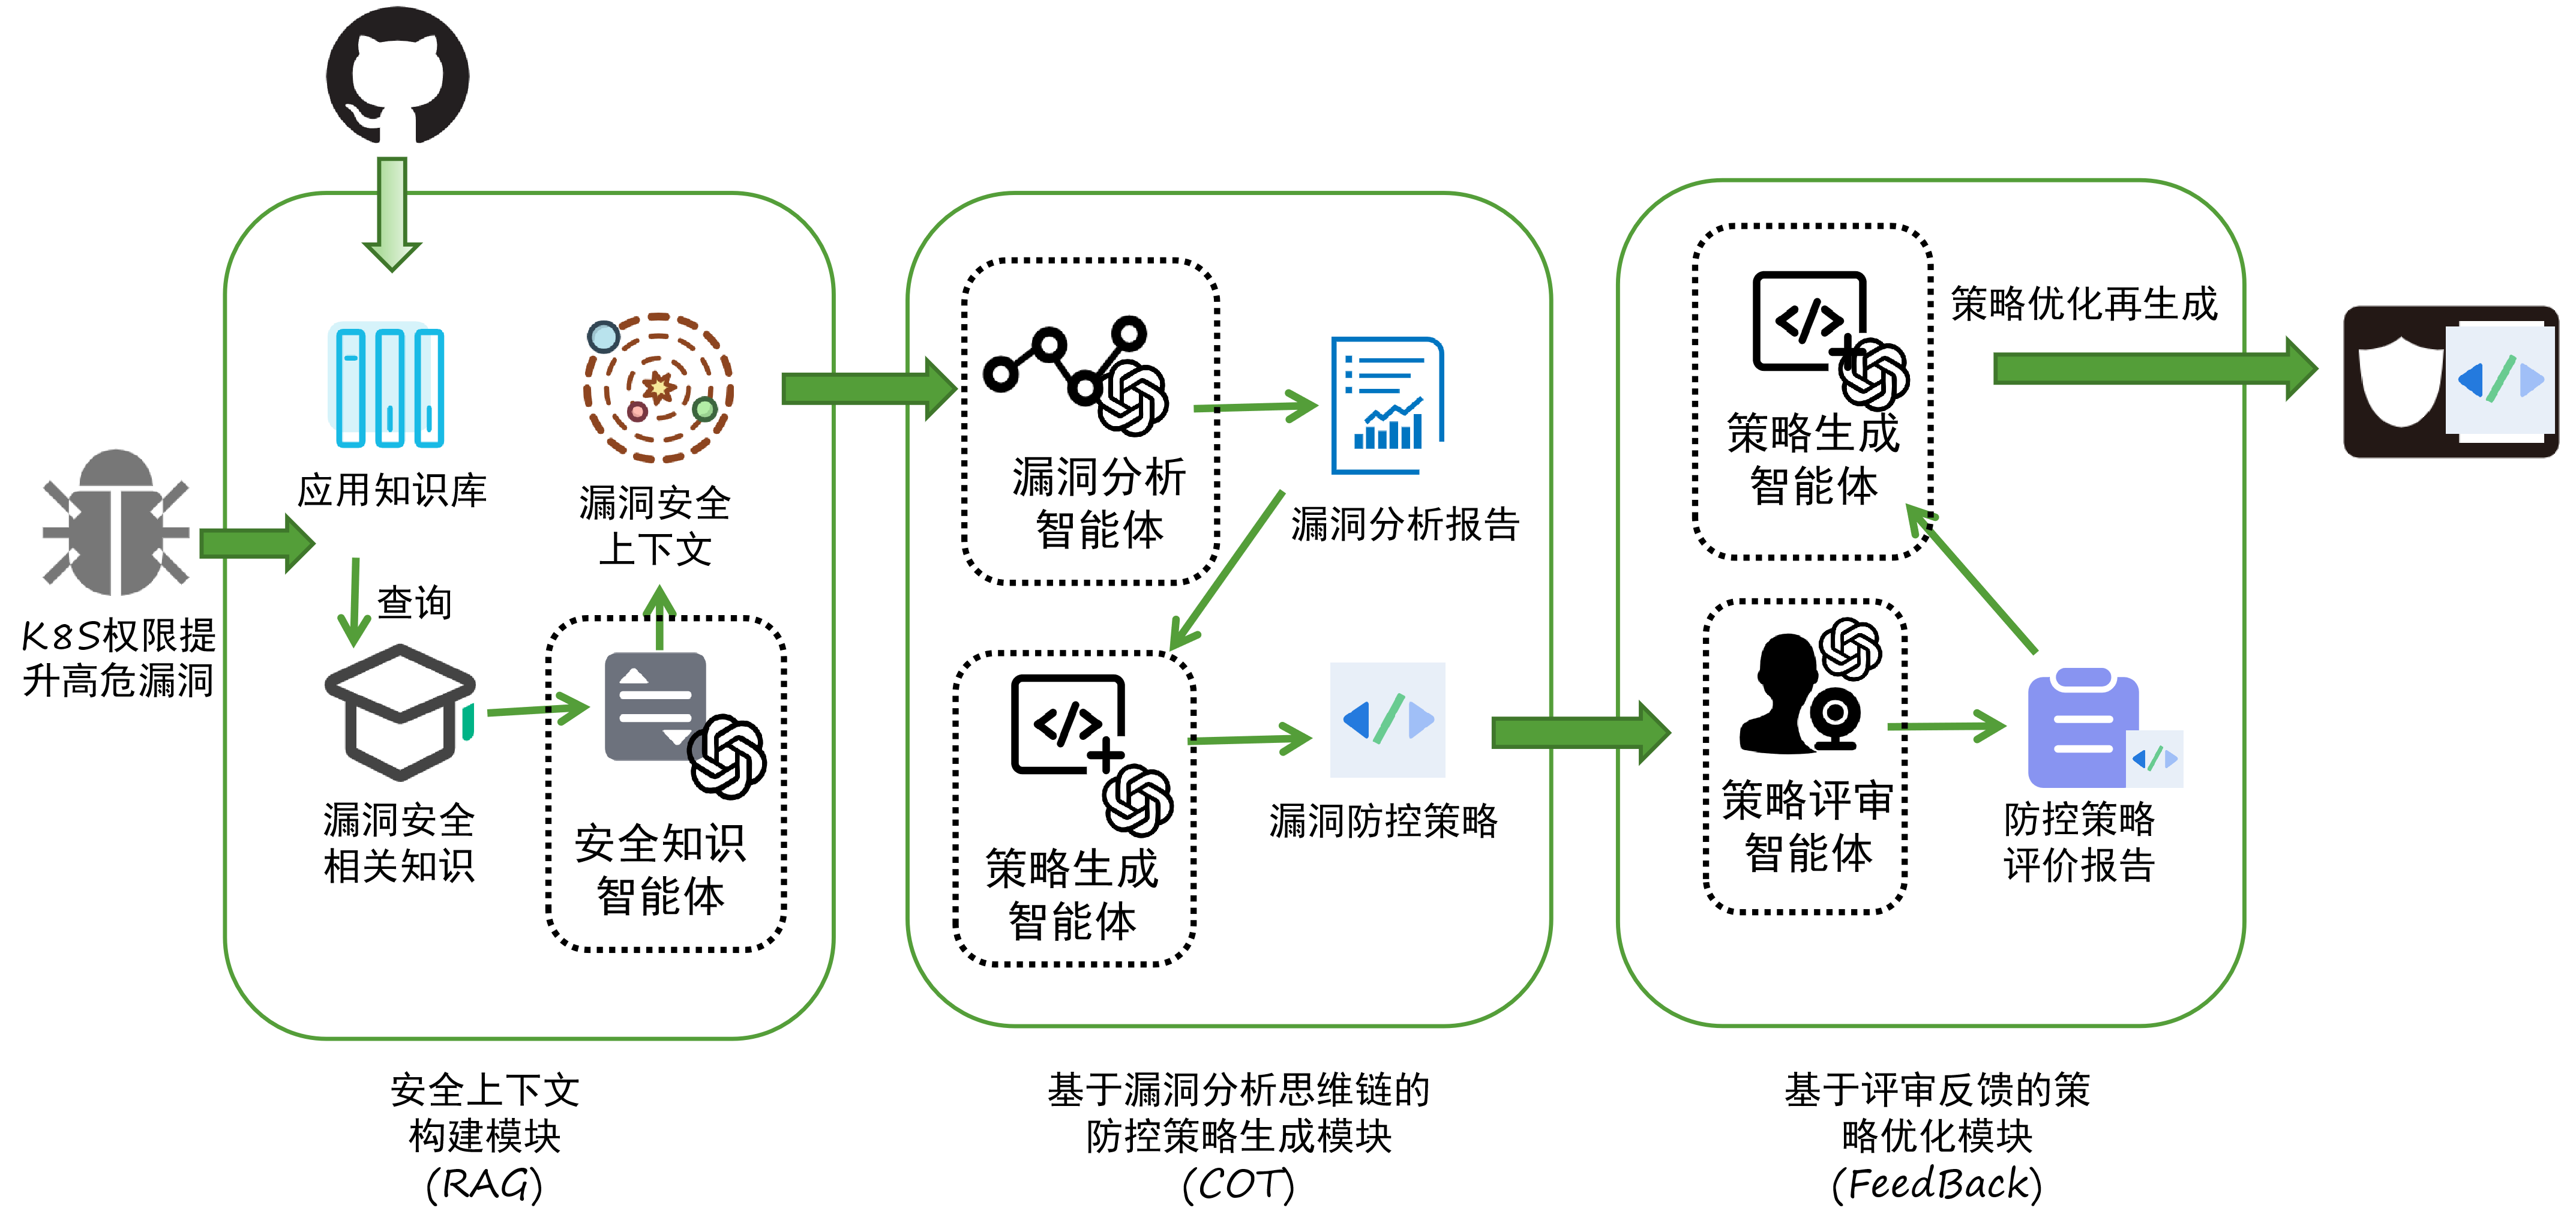
\includegraphics[width=1\textwidth]{images/method.png}
    \caption{智能安全策略生成框架}
    \label{fig:method}
\end{figure}


\subsection{安全上下文构建}

安全上下文构建以“证据可追溯”为目标，将漏洞相关信息组织为 $c=\{(t_i,\text{src}_i)\}_{i=1}^{n}$ 的证据集合。一方面，系统从应用知识库与安全材料中检索并汇聚候选证据（例如源代码、配置、文档、Issue、PR 与安全公告等），以兼顾覆盖度与召回精度；另一方面，引入\textbf{安全知识智能体}对检索结果进行二次整理：识别与 CVE 相关的关键事实（触发条件、受影响组件、权限边界与可控点等），并过滤与漏洞无关或重复的噪声片段。为支持后续复核与差异化处理，每条证据均保留来源标识与必要元数据；同时对冗余、超长或低质量文本进行裁剪与去重，避免上下文过载影响后续推导。

\subsection{基于漏洞分析思维链的策略生成}

该步骤在结构化约束下完成“漏洞分析—防控选型—策略生成”的顺序推导，并显式化关键中间结论，便于检查与复核。与仅输出自然语言建议不同，本文将中间产物与最终策略均约束为固定的 JSON 结构，从而降低信息缺失与表述歧义对交付的影响。

首先，\textbf{漏洞分析智能体}基于漏洞摘要与安全上下文 $c$ 输出结构化分析结果，覆盖漏洞类型、攻击向量、影响范围与风险等级，并给出与本文分类体系一致的风险类别。其次，\textbf{防控选型智能体}在分析结论的约束下，结合平台可用能力选择合适的控制手段（身份与权限、网络隔离、运行时安全与策略执行等），并给出实施思路与优先级。最后，\textbf{策略生成智能体}将上述结论汇总为最终策略 JSON，对关键字段、层级与顺序进行严格对齐；当信息不足以确定时，以 \texttt{(info needed)} 显式标注并给出必要假设。

为保证与本文形式化定义一致，策略内容采用 \texttt{layer/method/actions} 的表达方式：其中 \texttt{layer} 与 \texttt{method} 描述防控所在安全域与方法类别；\texttt{actions} 以可执行步骤序列承载具体控制措施。在工程化输出中，\texttt{actions} 可等价展开为策略 JSON 的 \texttt{mitigation.action} 字段，采用“1.. 2..”的步骤格式，并包含验证要点与回滚边界；当需要给出 YAML/CLI 片段时，统一使用转义换行 \texttt{\textbackslash n} 以保持 JSON 合法性。

\begin{itemize}
    \item \textbf{layer 字段}：防控所在的技术层面，用于分类防控策略所涉及的安全域，包括但不限于：
    \begin{itemize}
        \item 身份与权限：RBAC、认证强化、ServiceAccount管理等；
        \item 网络隔离：防火墙规则、NetworkPolicy、流量隔离等；
        \item 运行时检测：容器监控、系统调用检测、入侵检测等；
        \item 审计与日志：日志记录、事件审计、合规监控等。
    \end{itemize}
    \item \textbf{method 字段}：防控方法的摘要或分类，用于快速理解防控策略的整体思路，例如：
    \begin{itemize}
        \item 网络隔离与认证强化；
        \item 权限最小化与配置加固；
        \item 检测与阻断相结合。
    \end{itemize}
    \item \textbf{actions 字段}：具体可执行的操作序列，遵循定义3.1，包含：
    \begin{itemize}
        \item 对应的安全工具或修改对象（如Cisco DNA Center、Kubernetes RBAC配置）；
        \item 具体的执行步骤，包括命令、参数、验证方式；
        \item 副作用评估与回滚方案。
    \end{itemize}
\end{itemize}


为提高交付可用性，本文对候选策略施加基本质量要求：操作序列应可在短时间内启动；至少覆盖一个明确的防控层次；包含可验证的执行步骤；对潜在副作用与回滚边界作出清晰说明。

候选策略集合 $\Pi_v$ 的生成可采用多策略并行方法：对同一漏洞产生多个结构化策略对象，以探索不同的防控层次和防控方法。由于所有候选共享统一的 schema 结构（layer、method、actions），它们可直接进入后续的评价与排名流程。

在交付前，生成结果需进行规范化处理：统一各字段的格式、补齐缺失的操作步骤、清理冗余信息，并在数据缺失或不完整处显式标注假设条件和依赖的前置条件。

\subsection{基于评审反馈的策略优化}

该步骤通过“评审—反馈—再生成”的闭环对候选策略进行质量控制，以降低噪声与误报风险，并提升可部署性与一致性。具体而言，系统可并行生成多份候选策略形成 $\Pi_v$，随后由\textbf{策略评审智能体}对每份候选进行结构化评审，提炼有效控制点，指出潜在噪声来源（如误报概率高、运维负担过重或依赖条件不成立的配置），并给出上线前的验证需求与缺失信息清单。评审结论作为约束输入交由\textbf{策略优化智能体}进行二次整合：合并多份候选中被验证更可行的措施，剔除不可行或噪声过高的建议，补齐关键前置条件与回滚方案，并输出最终的优化策略。

在实现层面，本文将该过程与格式校验结合：若生成结果不满足 JSON 合法性或 schema 约束，则触发重试提示并要求按既定结构重新生成；优化阶段同时记录“改进主题—改进内容—来源候选”的对应关系，以便在复核时追踪优化依据与变化点。

\section{质量评价与筛选}

该阶段对候选策略集合进行结构化评价，输出门槛评分 $s(\pi)$、多维质量向量 $q(\pi)$ 和策略排名 $R(\Pi_v, \text{dim})$，遵循“结构化输入$\to$规则化检查$\to$证据支撑的结论”的流程，以提高结论的可验证性。

\subsection{门槛评分与质量评估}

评分函数 $s: \Pi \to [0,1]$ 用于判定策略是否满足最低可用性要求。该评分关注可部署性和风险降低效果。典型评价流程包括：

	\textbf{评价指标}。建立可核查的检查清单，包括：
\begin{itemize}
    \item 完整性检查（关键字段是否齐全，信息缺失是否标注）
    \item 可部署性检查（是否给出具体步骤、验证方法和回滚边界）
    \item 一致性检查（策略与安全上下文的一致性，是否包含无依据的断言）
    \item 约束合规检查（是否符合临时防控的适用范围）
\end{itemize}

	\textbf{评分聚合}。检查项结果通过加权和进行聚合：
\[
s(\pi)=\mathrm{clip}\left(\sum_{j=1}^{m} w_j\cdot r_j(\pi),\;0,\;1\right)
\]
其中 $r_j(\pi)$ 为第 $j$ 项的评分，$w_j$ 为权重。部分关键项可设置为硬约束，即任何关键项失败则整体评分低于阈值。

	\textbf{流程控制}。设定阈值 $\tau$，当 $s(\pi) < \tau$ 时策略转入反馈优化流程重新修订，当 $s(\pi) \geq \tau$ 时进入后续排名和筛选。

	\textbf{质量向量}。对通过门槛的策略，进一步用三维向量刻画其特性：
\[
q(\pi)=(E(\pi),\; I(\pi),\; D(\pi))
\]
其中：
\begin{itemize}
    \item $E(\pi)$：有效性，即覆盖关键攻击路径和降低风险的程度
    \item $I(\pi)$：干扰程度，即对业务运营、误报风险和运维复杂度的影响
    \item $D(\pi)$：可部署性，即步骤清晰度、可操作性和验证回滚能力
\end{itemize}

每个维度通过可观测指标聚合为 $[0,1]$ 分数，同时记录评分理由与证据来源。

\subsection{多维排名}

排名算子 $R(\Pi_v, \text{dim})$ 在指定维度上对候选策略进行排序：
\[
R(\Pi_v,\;\text{dim})\rightarrow(\pi_{(1)},\pi_{(2)},\ldots,\pi_{(k)})
\]

排名过程包括：
\begin{enumerate}
    \item \textbf{过滤}。移除评分低于阈值 $\tau$ 的候选，使后续排名的策略均可部署。
    \item \textbf{排序}。按指定维度（有效性、干扰程度或可部署性）的评分降序排列。
    \item \textbf{并列处理}。当分数接近时，引入次级准则（如降低干扰程度作为次级准则）。
    \item \textbf{结果说明}。输出排名序列及每个策略的三维评分、关键优缺点和支撑证据。
\end{enumerate}

\subsection{评价驱动的迭代控制}

评价结论决定策略是否可交付或需要进一步优化。当最高分候选仍低于阈值或关键维度存在缺陷时，评价报告转化为修订约束触发下一轮反馈优化；当候选达标时，按维度排名并输出支撑证据。

\section{LLM 生成的可靠性控制}

在以生成模型辅助策略构建的场景中，输出质量主要受三类因素影响：生成过程的随机性、输入证据的不完整性，以及对约束条件理解不一致带来的偏差。为提高结果的可复核性与可维护性，本文采用如下机制对输出进行“可检查化”约束：

\begin{enumerate}
    \item \textbf{结构化产物与字段检查}：将策略固定为（layer、method、actions）三字段对象；对字段完整性、格式一致性与动作序列可执行性进行规则化检查。
    
    \item \textbf{证据来源追踪}：对关键判断与关键配置项保留来源标识（文件路径、链接或片段 ID 等），使“结论—证据”可回溯。
    
    \item \textbf{分阶段输出与差异记录}：将推导过程拆分为可验证的中间输出，并在迭代修订时记录修改原因与变化点，便于定位问题来源。
    
    \item \textbf{多维评价与门槛控制}：通过门槛评分过滤明显不可部署的候选，再以质量向量进行排序，从而将主观判断转化为可比较的检查结果。
\end{enumerate}

上述机制的目标并非“消除不确定性”，而是将不确定性限定在可定位、可复核的范围内，使策略选择与交付过程具有一致的检查依据。

\section{实验设计与评估}

本节给出实验评估设置与结果展示。评估目标是检验本文提出的策略生成 pipeline 是否能够在多模型与多候选条件下，稳定产出可交付的临时防控策略，并为候选筛选提供一致的排名依据。此外，实验过程中也记录了不同方法的Token消耗与响应时间，以评估其在实际应用中的效率表现。

\subsection{实验设置}

实验使用五个大模型作为策略生成的基座模型：\texttt{Qwen3}、\texttt{DeepSeek}、\texttt{GPT-5}、\texttt{Grok} 与 \texttt{GLM-4.6}。对每个漏洞实例 $v$，系统在同一安全上下文 $c$ 下分别调用上述模型生成候选策略，形成候选集合 $\Pi_v$。为降低“单次生成偶然性”对结论的影响，评估以候选集合为对象进行对比与筛选，而不是仅报告单一候选。

\subsection{基于多模型互评的排名式评分}

在评审阶段，上述五个模型同时作为“评审者”对候选集合 $\Pi_v$ 进行排名式评分。评审指标沿用本文三维质量向量 $q(\pi)=(E(\pi),I(\pi),D(\pi))$：\textbf{有效性}（$E$）关注是否覆盖关键攻击路径并降低风险；\textbf{无干扰性}（$I$）关注对业务与运维的副作用、误报与额外复杂度；\textbf{可部署性}（$D$）关注步骤清晰度、可操作性，以及验证与回滚边界是否明确。

与直接给出绝对分数不同，评审者对每一维度输出候选策略的相对排序，并据此形成排名式评分结果。该设计的目的在于降低不同模型“分数尺度不一致”带来的偏差，使筛选过程更关注候选之间的相对优劣；同时，评审结论可与证据来源、前置条件与缺失信息清单共同输出，便于复核。

\subsection{结果展示}

图\ref{fig:single-dim-deployability}--图\ref{fig:single-dim-effectiveness} 展示了不同评审模型在三个单维度上的排名式评分结果，用于观察不同评审者对候选策略的偏好差异与一致性。

下面只展示了部分图标，完整结果请参见附录。

\begin{figure}[!ht]
    \centering
    {\setlength{\abovecaptionskip}{2pt}%
     \setlength{\belowcaptionskip}{0pt}%
     \subfloat[可部署性]{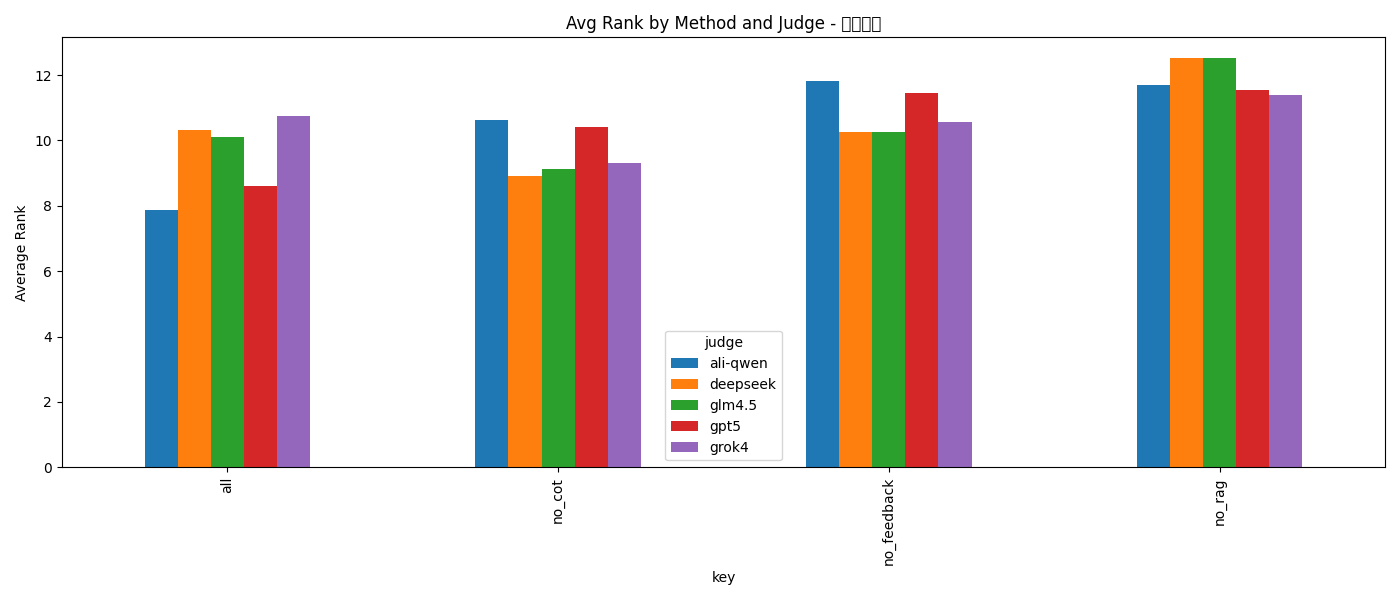
\includegraphics[width=0.95\textwidth]{images/plots/可部署性/summary/single_dim_by_judge_可部署性.png}\label{fig:single-dim-deployability}}\\[-2mm]
     \subfloat[无干扰性]{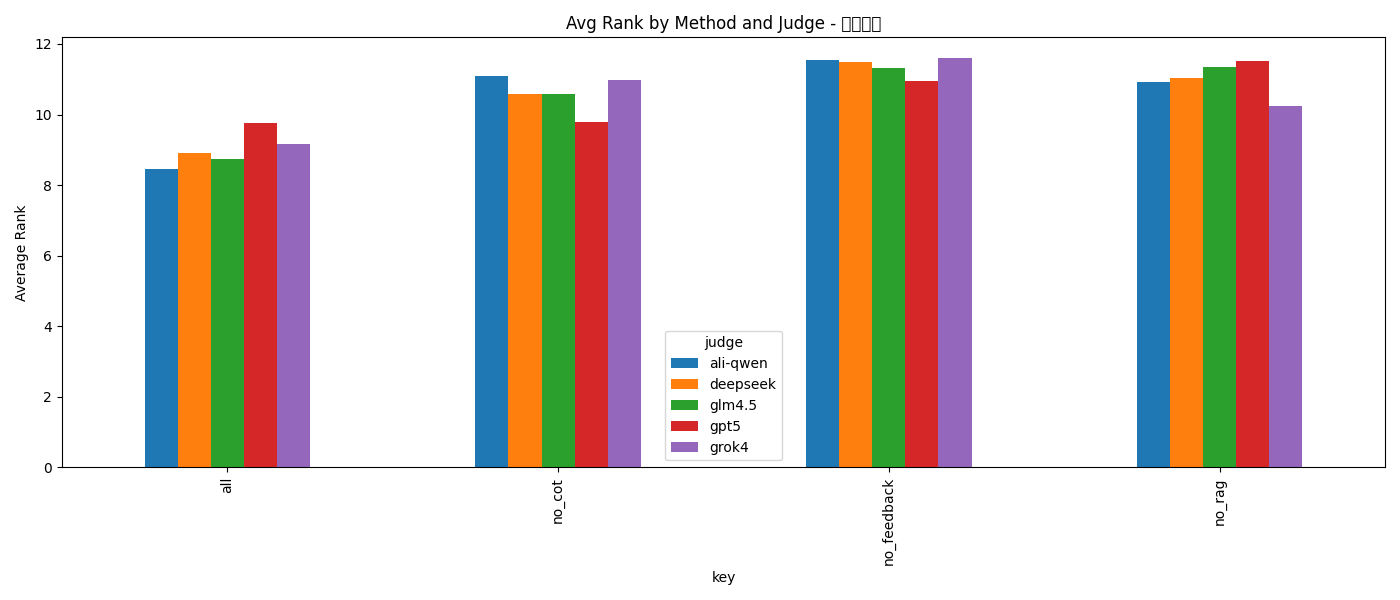
\includegraphics[width=0.95\textwidth]{images/plots/无干扰性/summary/single_dim_by_judge_无干扰性.png}\label{fig:single-dim-interference}}\\[-2mm]
     \subfloat[有效性]{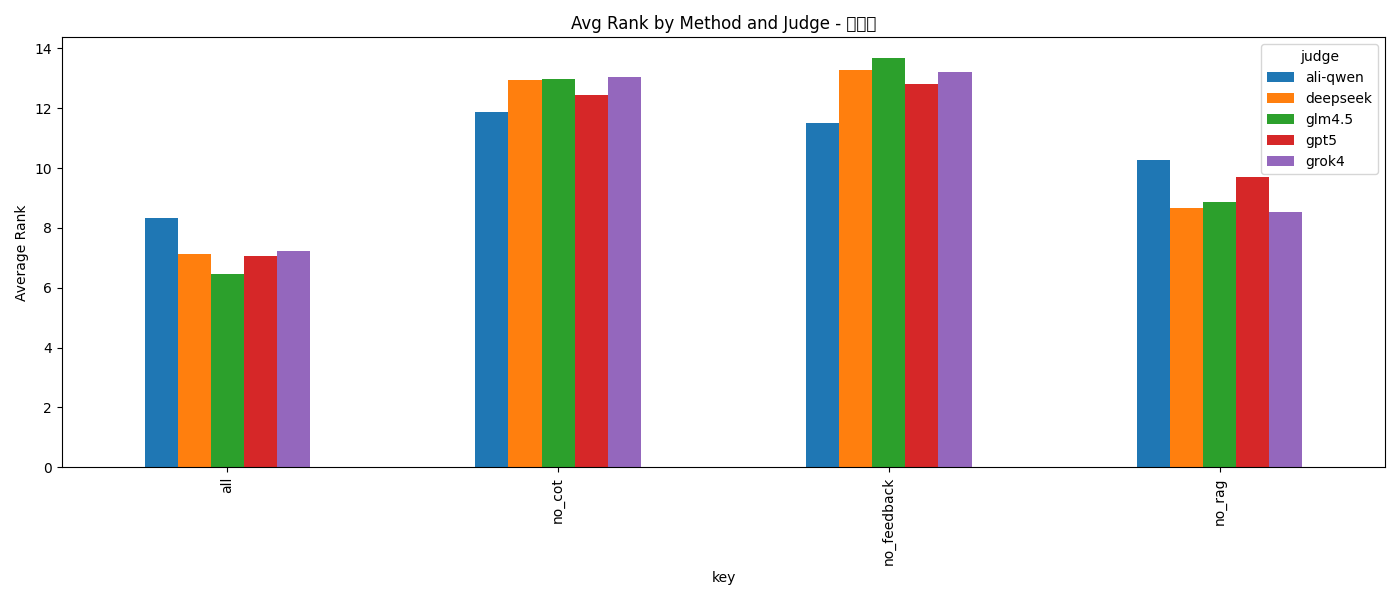
\includegraphics[width=0.95\textwidth]{images/plots/有效性/summary/single_dim_by_judge_有效性.png}\label{fig:single-dim-effectiveness}}}
    \caption{不同评审模型下的单维度排名式评分结果。}
\end{figure}


